\documentclass{article}
\usepackage[utf8]{inputenc}
\usepackage{authblk}
\usepackage{amsmath}
\usepackage{amssymb}
\usepackage{graphicx}
\usepackage{physics}
\usepackage{float}
\usepackage{bm}
\usepackage{caption}
\usepackage{subcaption}
\usepackage{dsfont}
\usepackage[parfill]{parskip}
\usepackage{blkarray}
\usepackage[dvipsnames]{xcolor}
\usepackage[most]{tcolorbox}

\newcommand{\Id}{\mathds{1}}
\newcommand\sj[1]{ {\color{orange} #1} } 


\newcommand{\matindex}[1]{\mbox{\scriptsize#1}}% Matrix index
\usepackage{geometry}
 \geometry{
 a4paper,
 left=25mm,
 right = 25 mm,
 top = 15mm,
 }


\title{QPC Project Status to 07.2025: Perturbative Approach}
\author{Santiago Salazar Jaramillo}
\date{}


\begin{document}
\maketitle

\section{First Order Corrections}

We consider the interaction between the QPC and the qubit to be the perturbative term. Therefore, the full Hamiltonian $H = H_0 + \Omega H_1$ is given by
\begin{align}
    H_0 = -\sum_{n}^{N}J(a_{n}^{\dagger} a_{n} + a_{n+1}^{\dagger}a_{n} ) - t(d_{1}^{\dagger}d_{0}+d_{0}^{\dagger}d_{1})
\end{align}
and 
\begin{align}
    H_1 = d_{1}^{\dagger}d_{1}( a_{b}^{\dagger}a_{b+1} + a^{\dagger}_{b+1}a_{b} )
\end{align}
where $a$, $d$ are the annihilation operators of the QPC and qubit respectively, and the sub-index $b$ refers to the QPC site where the bond is located. 

The eigenstates of $H_0$ are the tensor product $\ket{\phi^{(0)}_\nu (k)} = \ket{k}\otimes \ket{\nu}$, where $k$ is the label for the momentum states of the tight-binding model with open boundaries for the QPC, and $\nu = \pm$ refers to the symetric/anti-symmetric qubit states. 

\begin{tcolorbox}[title=QPC eigenstates, colback=white, colframe=black]
\begin{align}
    \bra{n}\ket{k} = \sqrt{\frac{1}{N+1}} \sin(n k) ,\quad & E(k) = -2J\cos(k), \quad k = \frac{n\pi}{N+1},\quad n= 1, 2,...N
\end{align}
Here $\ket{n}$ is the position basis.
\end{tcolorbox}

\begin{tcolorbox}[title=Qubit eigenstates, colback=white, colframe=black]
\begin{align}
   & \ket{+} = \frac{1}{\sqrt{2}}\left( \ket{0} + e^{i\phi} \ket{1}\right), \quad \epsilon_+ = t \\
   & \ket{-} = \frac{1}{\sqrt{2}}\left( \ket{0} - e^{i\phi} \ket{1}\right), \quad \epsilon_- = -t
\end{align}
\end{tcolorbox}

From this setup, the zeroth order energies are 
\begin{align}
   E_{\nu}(k)^{(0)} = E(k) + \epsilon_\nu = -2J\cos(k)\pm t,
\end{align}
meaning that, we now have two bands (symmetric anti-symmetric) of the tight-binding energy spectrum.

The following matrix element often appears in the later calculations
\begin{align}
    \bra{\phi^{(0)}_\mu (p)}H_1 \ket{\phi^{(0)}_\nu (k)} = \bra{\mu}d^\dagger_0 d_0 \ket{\nu} \bra{p}\left( a_{b}^{\dagger}a_{b+1} + a^{\dagger}_{b+1}a_{b}  \right) \ket{k}.
\end{align}
The momentum part can be calculated by changing to the lattice basis by inserting $1 = \sum_{n} \ket{n}\bra{n}$ two times and resolving the orthogonality conditions
\begin{align}
    \bra{\phi^{(0)}_\mu (p)}H_1 \ket{\phi^{(0)}_\nu (k)} = \frac{1}{N+1} \left(  \sin(bk+k)\sin(bp)+ \sin(bp+p)\sin(bk)\right) = \frac{1}{N+1} \xi(k,p).
\end{align}
Notice that, since the interaction is local, only the sites near the bond contribute. 
In addition, this form makes it explicit that the perturbation couples the occupation 
at the state $\ket{0}$ of the qubit with the momentum of the QPC particle.

The first order corrections to the energy are
\begin{align}
    E_{\nu}^{(1)}(k) = \bra{\phi^{(0)}_\nu (k)}H_1 \ket{\phi^{(0)}_\nu (k)} = \frac{1}{N+1} \xi(k,k).
\end{align}
Hence, to first order both bands are affected equally and due to the periodicity of 
$\xi(k,k)$ some energy states will not change, as is seen in figure \ref{fig:E1}.

\begin{figure*}[h!]
    \centering
        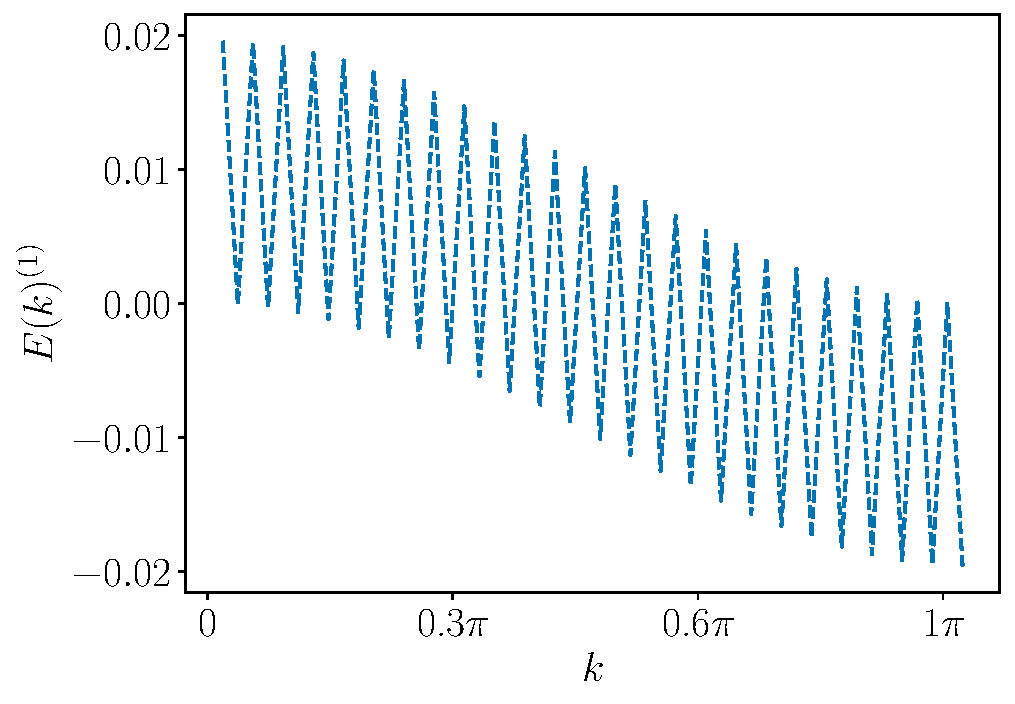
\includegraphics[width=0.5\linewidth]{figures/report_07_2025/E1_corr=50_Omega=0.5_t=0.4.pdf}
        \caption{First order corrections to the energy for a system with 50 sites in the QPC.}
\end{figure*}\label{fig:E1}

The second order corrections are given by 
\begin{align}
    E_{\nu}^{(2)}(k) & = \sum_{(\mu,p)\neq(\nu,k)} \frac{\left|\bra{\phi^{(0)}_\mu (p)}H_1 \ket{\phi^{(0)}_\nu (k)}\right|^2}{ E_{\nu}^{(0)}(k) -  E_{\mu}^{(0)}(p)}\\
    & = \frac{1}{(N+1)^2}\sum_{(\mu,p)\neq(\nu,k)} \frac{ \xi(k,p)^2}{ E_{\nu}^{(0)}(k) -  E_{\mu}^{(0)}(p)}
\end{align}
where the summation over the $\mu$ and $p$ states is subject to the condition that 
both cannot be equal to $\nu$ and $k$ at the same time. To simplify the calculation,
 it is convenient to separate the sum into three terms
\begin{align}\label{eq:E2}
    E_{\nu}^{(2)}(k) & = \frac{1}{(N+1)^2}\sum_{p\neq k} \left \{ \frac{ \xi(k,p)^2}{ -2J( \cos k - \cos p ) } +  \frac{ \xi(k,p)^2}{ 2\epsilon_\nu -2J( \cos k - \cos p ) } \right \} + \frac{1}{(N+1)^2} \frac{\xi(k,k)^2}{2\epsilon_\nu},
\end{align}
where the first term corresponds to $\mu = \nu, p\neq k$, the second to $\mu \neq \nu, p\neq k$ and the third to $\mu \neq \nu, p = k$. Notice that there are some degeneracies in this expression, when $k$ gets close to the $0, \pi$  boundaries of the band and when $\epsilon_\nu = -2 J( \cos k -\cos p)$. We shall discuss these in the following after calculating the corrections to the eigenstates as the meaning will be clearer there. 

The first order corrections to the eigenstates are
\begin{align}
    \ket{\phi_\nu^{(1)} (k)} = \sum_{(\mu,p)\neq(\nu,k)} \frac{\bra{\phi^{(0)}_\mu (p)}H_1 \ket{\phi^{(0)}_\nu (k)}}{ E_{\nu}^{(0)}(k) -  E_{\mu}^{(0)}(p)} \ket{p}\otimes \ket{\mu}.
\end{align} 
Much like with the energy, it is convenient to separate the sums into three following three terms
\begin{align}\label{eq:psi_1}
    \ket{\phi_\nu^{(1)} (k)} = & \frac{1}{(N+1)}\sum_{p\neq k} \ket{p}\otimes \left \{ \frac{ \xi(k,p)}{ -2J( \cos k - \cos p ) } \ket{\nu} +  \frac{ \xi(k,p)^2}{ 2\epsilon_\nu -2J( \cos k - \cos p )} \ket{\mu} \right \} \nonumber \\ 
    & + \frac{1}{(N+1)} \frac{\xi(k,k)}{2\epsilon_\nu} \ket{k}\otimes\ket{\mu},
\end{align}
corresponding to the same ones from Eq.\eqref{eq:E2}. Here, it is important to point out the convention that $\mu \neq \nu$ when it appears explicitly in such a form. This convention is held for the rest of this text.

Now, working with Eq.\eqref{eq:psi_1} it is easier to understand what the aforementioned degeneracies mean. The first term, mixes momentum states within the same band and becomes degenerate towards the edges ($k\approx 0, \pi$) due to the cosine shape of the energy levels. 

On the other hand, the second term is more interesting. It mixes momentum states from different bands ($\nu$ and $\mu$), and becomes degenerate when the difference of between the QPC energies is equal to the band-gap, which can happen at several momenta. If $\nu = +$ the denominator blows up at $p=\pm \arccos(-t/J + \cos k)$ and for $\nu = -$ it happens at $p=\pm \arccos(t/J + \cos k)$. The dependence on the $\arccos$ imposes additional restrictions to the momenta that can cause a degeneracy. Since it is only defined for an argument between $-1$ and $1$, the only states that contribute are those that fulfill
\begin{align}
    -1 + \frac{t}{J} < \cos k < 1 - \frac{t}{J}.
\end{align}
This condition implies that, at larger values of $t$, there will be less available states that can become degenerate and hybridize the two bands. 

Furthermore, in order to guarantee that the perturbative expansion is well defined one has

\subsection{Corrections to the Reduced Density Matrix}


\bibliography{qpc}
\bibliographystyle{ieeetr}


\end{document}